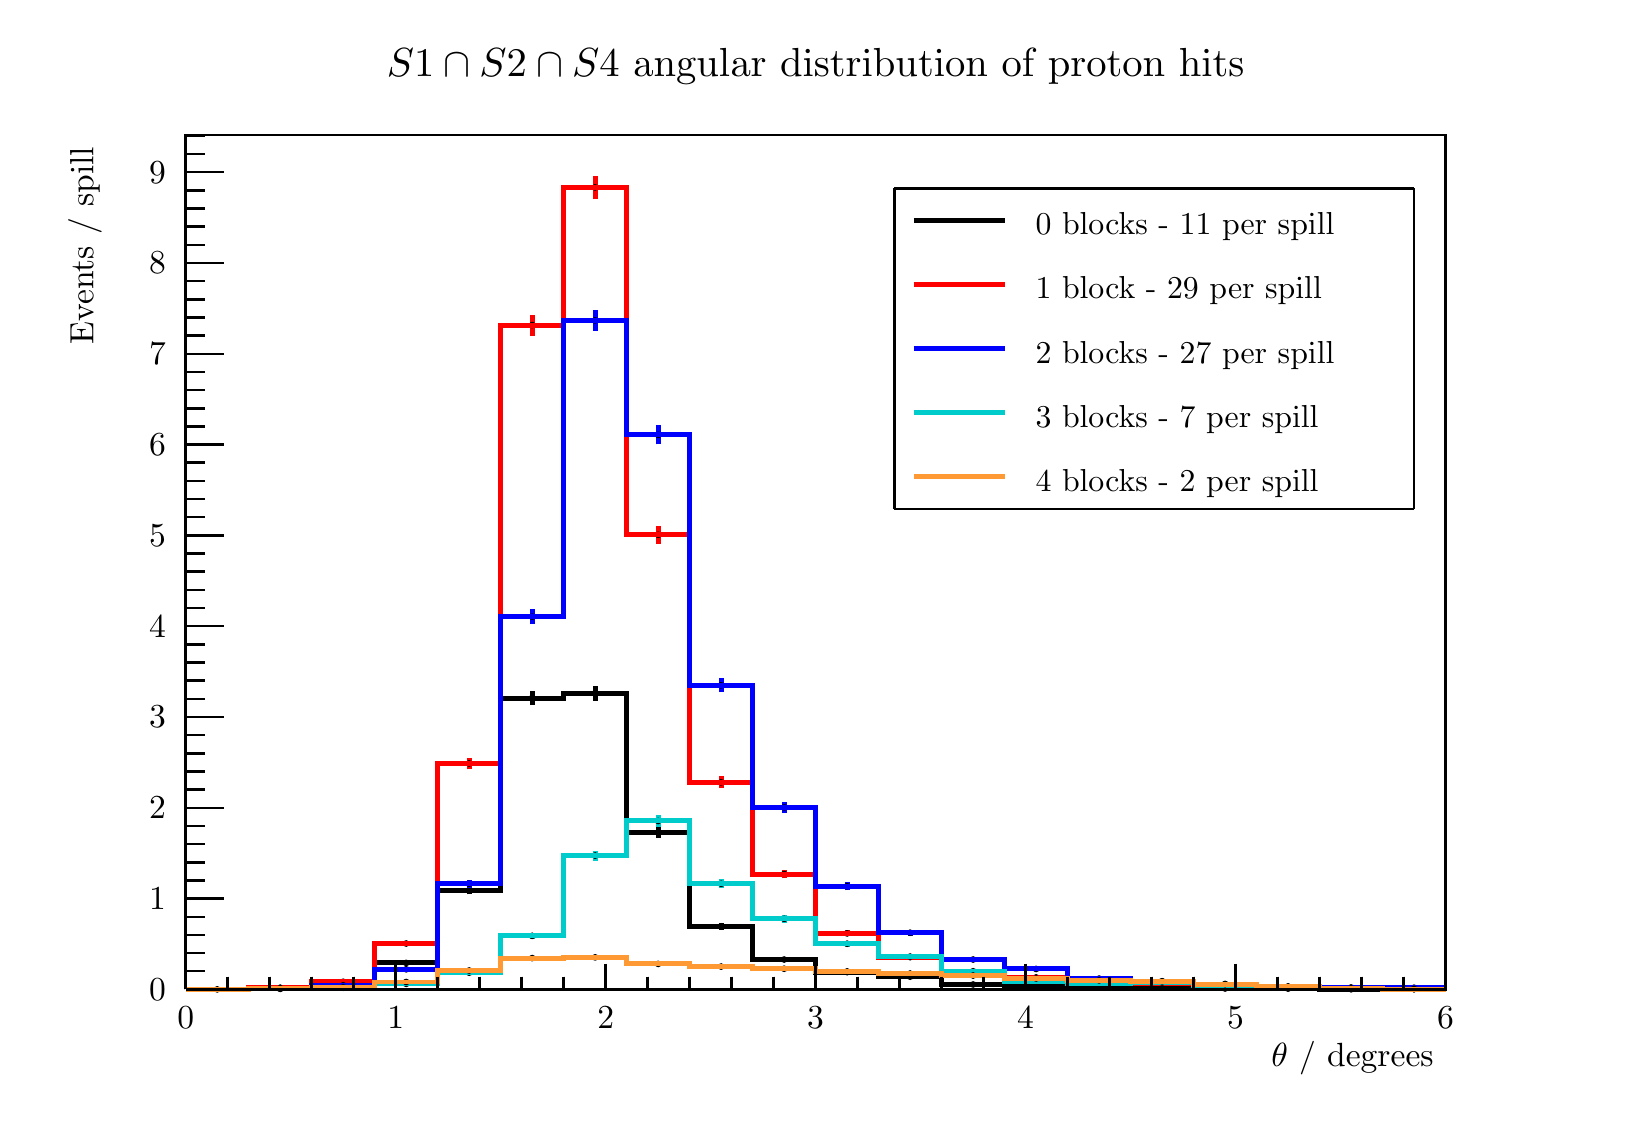
\begin{tikzpicture}
\pgfdeclareplotmark{cross} {
\pgfpathmoveto{\pgfpoint{-0.3\pgfplotmarksize}{\pgfplotmarksize}}
\pgfpathlineto{\pgfpoint{+0.3\pgfplotmarksize}{\pgfplotmarksize}}
\pgfpathlineto{\pgfpoint{+0.3\pgfplotmarksize}{0.3\pgfplotmarksize}}
\pgfpathlineto{\pgfpoint{+1\pgfplotmarksize}{0.3\pgfplotmarksize}}
\pgfpathlineto{\pgfpoint{+1\pgfplotmarksize}{-0.3\pgfplotmarksize}}
\pgfpathlineto{\pgfpoint{+0.3\pgfplotmarksize}{-0.3\pgfplotmarksize}}
\pgfpathlineto{\pgfpoint{+0.3\pgfplotmarksize}{-1.\pgfplotmarksize}}
\pgfpathlineto{\pgfpoint{-0.3\pgfplotmarksize}{-1.\pgfplotmarksize}}
\pgfpathlineto{\pgfpoint{-0.3\pgfplotmarksize}{-0.3\pgfplotmarksize}}
\pgfpathlineto{\pgfpoint{-1.\pgfplotmarksize}{-0.3\pgfplotmarksize}}
\pgfpathlineto{\pgfpoint{-1.\pgfplotmarksize}{0.3\pgfplotmarksize}}
\pgfpathlineto{\pgfpoint{-0.3\pgfplotmarksize}{0.3\pgfplotmarksize}}
\pgfpathclose
\pgfusepathqstroke
}
\pgfdeclareplotmark{cross*} {
\pgfpathmoveto{\pgfpoint{-0.3\pgfplotmarksize}{\pgfplotmarksize}}
\pgfpathlineto{\pgfpoint{+0.3\pgfplotmarksize}{\pgfplotmarksize}}
\pgfpathlineto{\pgfpoint{+0.3\pgfplotmarksize}{0.3\pgfplotmarksize}}
\pgfpathlineto{\pgfpoint{+1\pgfplotmarksize}{0.3\pgfplotmarksize}}
\pgfpathlineto{\pgfpoint{+1\pgfplotmarksize}{-0.3\pgfplotmarksize}}
\pgfpathlineto{\pgfpoint{+0.3\pgfplotmarksize}{-0.3\pgfplotmarksize}}
\pgfpathlineto{\pgfpoint{+0.3\pgfplotmarksize}{-1.\pgfplotmarksize}}
\pgfpathlineto{\pgfpoint{-0.3\pgfplotmarksize}{-1.\pgfplotmarksize}}
\pgfpathlineto{\pgfpoint{-0.3\pgfplotmarksize}{-0.3\pgfplotmarksize}}
\pgfpathlineto{\pgfpoint{-1.\pgfplotmarksize}{-0.3\pgfplotmarksize}}
\pgfpathlineto{\pgfpoint{-1.\pgfplotmarksize}{0.3\pgfplotmarksize}}
\pgfpathlineto{\pgfpoint{-0.3\pgfplotmarksize}{0.3\pgfplotmarksize}}
\pgfpathclose
\pgfusepathqfillstroke
}
\pgfdeclareplotmark{newstar} {
\pgfpathmoveto{\pgfqpoint{0pt}{\pgfplotmarksize}}
\pgfpathlineto{\pgfqpointpolar{44}{0.5\pgfplotmarksize}}
\pgfpathlineto{\pgfqpointpolar{18}{\pgfplotmarksize}}
\pgfpathlineto{\pgfqpointpolar{-20}{0.5\pgfplotmarksize}}
\pgfpathlineto{\pgfqpointpolar{-54}{\pgfplotmarksize}}
\pgfpathlineto{\pgfqpointpolar{-90}{0.5\pgfplotmarksize}}
\pgfpathlineto{\pgfqpointpolar{234}{\pgfplotmarksize}}
\pgfpathlineto{\pgfqpointpolar{198}{0.5\pgfplotmarksize}}
\pgfpathlineto{\pgfqpointpolar{162}{\pgfplotmarksize}}
\pgfpathlineto{\pgfqpointpolar{134}{0.5\pgfplotmarksize}}
\pgfpathclose
\pgfusepathqstroke
}
\pgfdeclareplotmark{newstar*} {
\pgfpathmoveto{\pgfqpoint{0pt}{\pgfplotmarksize}}
\pgfpathlineto{\pgfqpointpolar{44}{0.5\pgfplotmarksize}}
\pgfpathlineto{\pgfqpointpolar{18}{\pgfplotmarksize}}
\pgfpathlineto{\pgfqpointpolar{-20}{0.5\pgfplotmarksize}}
\pgfpathlineto{\pgfqpointpolar{-54}{\pgfplotmarksize}}
\pgfpathlineto{\pgfqpointpolar{-90}{0.5\pgfplotmarksize}}
\pgfpathlineto{\pgfqpointpolar{234}{\pgfplotmarksize}}
\pgfpathlineto{\pgfqpointpolar{198}{0.5\pgfplotmarksize}}
\pgfpathlineto{\pgfqpointpolar{162}{\pgfplotmarksize}}
\pgfpathlineto{\pgfqpointpolar{134}{0.5\pgfplotmarksize}}
\pgfpathclose
\pgfusepathqfillstroke
}
\definecolor{c}{rgb}{1,1,1};
\draw [color=c, fill=c] (0,0) rectangle (20,13.5632);
\draw [color=c, fill=c] (2,1.35632) rectangle (18,12.2069);
\definecolor{c}{rgb}{0,0,0};
\draw [c,line width=0.9] (2,1.35632) -- (2,12.2069) -- (18,12.2069) -- (18,1.35632) -- (2,1.35632);
\definecolor{c}{rgb}{1,1,1};
\draw [color=c, fill=c] (2,1.35632) rectangle (18,12.2069);
\definecolor{c}{rgb}{0,0,0};
\draw [c,line width=0.9] (2,1.35632) -- (2,12.2069) -- (18,12.2069) -- (18,1.35632) -- (2,1.35632);
\definecolor{c}{rgb}{0,0,0.6};
\draw [c,line width=0.9] (2,1.35632) -- (2.8,1.35632) -- (2.8,1.35632) -- (3.6,1.35632) -- (3.6,1.35632) -- (4.4,1.35632) -- (4.4,1.35632) -- (5.2,1.35632) -- (5.2,1.35632) -- (6,1.35632) -- (6,1.35632) -- (6.8,1.35632) -- (6.8,1.35632) --
 (7.6,1.35632) -- (7.6,1.35632) -- (8.4,1.35632) -- (8.4,1.35632) -- (9.2,1.35632) -- (9.2,1.35632) -- (10,1.35632) -- (10,1.35632) -- (10.8,1.35632) -- (10.8,1.35632) -- (11.6,1.35632) -- (11.6,1.35632) -- (12.4,1.35632) -- (12.4,1.35632) --
 (13.2,1.35632) -- (13.2,1.35632) -- (14,1.35632) -- (14,1.35632) -- (14.8,1.35632) -- (14.8,1.35632) -- (15.6,1.35632) -- (15.6,1.35632) -- (16.4,1.35632) -- (16.4,1.35632) -- (17.2,1.35632) -- (17.2,1.35632) -- (18,1.35632);
\definecolor{c}{rgb}{0,0,0};
\draw [c,line width=0.9] (2,1.35632) -- (18,1.35632);
\draw [anchor= east] (18,0.488276) node[scale=1.2126, color=c, rotate=0]{$\theta$ / degrees};
\draw [c,line width=0.9] (2,1.68184) -- (2,1.35632);
\draw [c,line width=0.9] (2.53333,1.51908) -- (2.53333,1.35632);
\draw [c,line width=0.9] (3.06667,1.51908) -- (3.06667,1.35632);
\draw [c,line width=0.9] (3.6,1.51908) -- (3.6,1.35632);
\draw [c,line width=0.9] (4.13333,1.51908) -- (4.13333,1.35632);
\draw [c,line width=0.9] (4.66667,1.68184) -- (4.66667,1.35632);
\draw [c,line width=0.9] (5.2,1.51908) -- (5.2,1.35632);
\draw [c,line width=0.9] (5.73333,1.51908) -- (5.73333,1.35632);
\draw [c,line width=0.9] (6.26667,1.51908) -- (6.26667,1.35632);
\draw [c,line width=0.9] (6.8,1.51908) -- (6.8,1.35632);
\draw [c,line width=0.9] (7.33333,1.68184) -- (7.33333,1.35632);
\draw [c,line width=0.9] (7.86667,1.51908) -- (7.86667,1.35632);
\draw [c,line width=0.9] (8.4,1.51908) -- (8.4,1.35632);
\draw [c,line width=0.9] (8.93333,1.51908) -- (8.93333,1.35632);
\draw [c,line width=0.9] (9.46667,1.51908) -- (9.46667,1.35632);
\draw [c,line width=0.9] (10,1.68184) -- (10,1.35632);
\draw [c,line width=0.9] (10.5333,1.51908) -- (10.5333,1.35632);
\draw [c,line width=0.9] (11.0667,1.51908) -- (11.0667,1.35632);
\draw [c,line width=0.9] (11.6,1.51908) -- (11.6,1.35632);
\draw [c,line width=0.9] (12.1333,1.51908) -- (12.1333,1.35632);
\draw [c,line width=0.9] (12.6667,1.68184) -- (12.6667,1.35632);
\draw [c,line width=0.9] (13.2,1.51908) -- (13.2,1.35632);
\draw [c,line width=0.9] (13.7333,1.51908) -- (13.7333,1.35632);
\draw [c,line width=0.9] (14.2667,1.51908) -- (14.2667,1.35632);
\draw [c,line width=0.9] (14.8,1.51908) -- (14.8,1.35632);
\draw [c,line width=0.9] (15.3333,1.68184) -- (15.3333,1.35632);
\draw [c,line width=0.9] (15.8667,1.51908) -- (15.8667,1.35632);
\draw [c,line width=0.9] (16.4,1.51908) -- (16.4,1.35632);
\draw [c,line width=0.9] (16.9333,1.51908) -- (16.9333,1.35632);
\draw [c,line width=0.9] (17.4667,1.51908) -- (17.4667,1.35632);
\draw [c,line width=0.9] (18,1.68184) -- (18,1.35632);
\draw [anchor=base] (2,0.854483) node[scale=1.2126, color=c, rotate=0]{0};
\draw [anchor=base] (4.66667,0.854483) node[scale=1.2126, color=c, rotate=0]{1};
\draw [anchor=base] (7.33333,0.854483) node[scale=1.2126, color=c, rotate=0]{2};
\draw [anchor=base] (10,0.854483) node[scale=1.2126, color=c, rotate=0]{3};
\draw [anchor=base] (12.6667,0.854483) node[scale=1.2126, color=c, rotate=0]{4};
\draw [anchor=base] (15.3333,0.854483) node[scale=1.2126, color=c, rotate=0]{5};
\draw [anchor=base] (18,0.854483) node[scale=1.2126, color=c, rotate=0]{6};
\draw [c,line width=0.9] (2,1.35632) -- (2,12.2069);
\draw [anchor= east] (0.72,12.2069) node[scale=1.2126, color=c, rotate=90]{ Events / spill};
\draw [c,line width=0.9] (2.48,1.35632) -- (2,1.35632);
\draw [c,line width=0.9] (2.24,1.58696) -- (2,1.58696);
\draw [c,line width=0.9] (2.24,1.81759) -- (2,1.81759);
\draw [c,line width=0.9] (2.24,2.04823) -- (2,2.04823);
\draw [c,line width=0.9] (2.24,2.27886) -- (2,2.27886);
\draw [c,line width=0.9] (2.48,2.5095) -- (2,2.5095);
\draw [c,line width=0.9] (2.24,2.74013) -- (2,2.74013);
\draw [c,line width=0.9] (2.24,2.97077) -- (2,2.97077);
\draw [c,line width=0.9] (2.24,3.20141) -- (2,3.20141);
\draw [c,line width=0.9] (2.24,3.43204) -- (2,3.43204);
\draw [c,line width=0.9] (2.48,3.66268) -- (2,3.66268);
\draw [c,line width=0.9] (2.24,3.89331) -- (2,3.89331);
\draw [c,line width=0.9] (2.24,4.12395) -- (2,4.12395);
\draw [c,line width=0.9] (2.24,4.35458) -- (2,4.35458);
\draw [c,line width=0.9] (2.24,4.58522) -- (2,4.58522);
\draw [c,line width=0.9] (2.48,4.81585) -- (2,4.81585);
\draw [c,line width=0.9] (2.24,5.04649) -- (2,5.04649);
\draw [c,line width=0.9] (2.24,5.27712) -- (2,5.27712);
\draw [c,line width=0.9] (2.24,5.50776) -- (2,5.50776);
\draw [c,line width=0.9] (2.24,5.7384) -- (2,5.7384);
\draw [c,line width=0.9] (2.48,5.96903) -- (2,5.96903);
\draw [c,line width=0.9] (2.24,6.19967) -- (2,6.19967);
\draw [c,line width=0.9] (2.24,6.4303) -- (2,6.4303);
\draw [c,line width=0.9] (2.24,6.66094) -- (2,6.66094);
\draw [c,line width=0.9] (2.24,6.89157) -- (2,6.89157);
\draw [c,line width=0.9] (2.48,7.12221) -- (2,7.12221);
\draw [c,line width=0.9] (2.24,7.35284) -- (2,7.35284);
\draw [c,line width=0.9] (2.24,7.58348) -- (2,7.58348);
\draw [c,line width=0.9] (2.24,7.81412) -- (2,7.81412);
\draw [c,line width=0.9] (2.24,8.04475) -- (2,8.04475);
\draw [c,line width=0.9] (2.48,8.27539) -- (2,8.27539);
\draw [c,line width=0.9] (2.24,8.50602) -- (2,8.50602);
\draw [c,line width=0.9] (2.24,8.73666) -- (2,8.73666);
\draw [c,line width=0.9] (2.24,8.96729) -- (2,8.96729);
\draw [c,line width=0.9] (2.24,9.19793) -- (2,9.19793);
\draw [c,line width=0.9] (2.48,9.42856) -- (2,9.42856);
\draw [c,line width=0.9] (2.24,9.6592) -- (2,9.6592);
\draw [c,line width=0.9] (2.24,9.88983) -- (2,9.88983);
\draw [c,line width=0.9] (2.24,10.1205) -- (2,10.1205);
\draw [c,line width=0.9] (2.24,10.3511) -- (2,10.3511);
\draw [c,line width=0.9] (2.48,10.5817) -- (2,10.5817);
\draw [c,line width=0.9] (2.24,10.8124) -- (2,10.8124);
\draw [c,line width=0.9] (2.24,11.043) -- (2,11.043);
\draw [c,line width=0.9] (2.24,11.2736) -- (2,11.2736);
\draw [c,line width=0.9] (2.24,11.5043) -- (2,11.5043);
\draw [c,line width=0.9] (2.48,11.7349) -- (2,11.7349);
\draw [c,line width=0.9] (2.48,11.7349) -- (2,11.7349);
\draw [c,line width=0.9] (2.24,11.9656) -- (2,11.9656);
\draw [c,line width=0.9] (2.24,12.1962) -- (2,12.1962);
\draw [anchor= east] (1.9,1.35632) node[scale=1.2126, color=c, rotate=0]{0};
\draw [anchor= east] (1.9,2.5095) node[scale=1.2126, color=c, rotate=0]{1};
\draw [anchor= east] (1.9,3.66268) node[scale=1.2126, color=c, rotate=0]{2};
\draw [anchor= east] (1.9,4.81585) node[scale=1.2126, color=c, rotate=0]{3};
\draw [anchor= east] (1.9,5.96903) node[scale=1.2126, color=c, rotate=0]{4};
\draw [anchor= east] (1.9,7.12221) node[scale=1.2126, color=c, rotate=0]{5};
\draw [anchor= east] (1.9,8.27539) node[scale=1.2126, color=c, rotate=0]{6};
\draw [anchor= east] (1.9,9.42856) node[scale=1.2126, color=c, rotate=0]{7};
\draw [anchor= east] (1.9,10.5817) node[scale=1.2126, color=c, rotate=0]{8};
\draw [anchor= east] (1.9,11.7349) node[scale=1.2126, color=c, rotate=0]{9};
\draw [c,line width=1.8] (3.2,1.36907) -- (3.2,1.3733);
\draw [c,line width=1.8] (3.2,1.3733) -- (3.2,1.37753);
\foreach \P in {(3.2,1.3733)}{\draw[mark options={color=c,fill=c},mark size=2.402402pt,mark=*,mark size=1pt] plot coordinates {\P};}
\draw [c,line width=1.8] (4,1.42823) -- (4,1.43742);
\draw [c,line width=1.8] (4,1.43742) -- (4,1.44661);
\foreach \P in {(4,1.43742)}{\draw[mark options={color=c,fill=c},mark size=2.402402pt,mark=*,mark size=1pt] plot coordinates {\P};}
\draw [c,line width=1.8] (4.8,1.67212) -- (4.8,1.6928);
\draw [c,line width=1.8] (4.8,1.6928) -- (4.8,1.71347);
\foreach \P in {(4.8,1.6928)}{\draw[mark options={color=c,fill=c},mark size=2.402402pt,mark=*,mark size=1pt] plot coordinates {\P};}
\draw [c,line width=1.8] (5.6,2.56355) -- (5.6,2.61121);
\draw [c,line width=1.8] (5.6,2.61121) -- (5.6,2.65886);
\foreach \P in {(5.6,2.61121)}{\draw[mark options={color=c,fill=c},mark size=2.402402pt,mark=*,mark size=1pt] plot coordinates {\P};}
\draw [c,line width=1.8] (6.4,4.96678) -- (6.4,5.05684);
\draw [c,line width=1.8] (6.4,5.05684) -- (6.4,5.14691);
\foreach \P in {(6.4,5.05684)}{\draw[mark options={color=c,fill=c},mark size=2.402402pt,mark=*,mark size=1pt] plot coordinates {\P};}
\draw [c,line width=1.8] (7.2,5.02241) -- (7.2,5.11701);
\draw [c,line width=1.8] (7.2,5.11701) -- (7.2,5.2116);
\foreach \P in {(7.2,5.11701)}{\draw[mark options={color=c,fill=c},mark size=2.402402pt,mark=*,mark size=1pt] plot coordinates {\P};}
\draw [c,line width=1.8] (8,3.28178) -- (8,3.34989);
\draw [c,line width=1.8] (8,3.34989) -- (8,3.41799);
\foreach \P in {(8,3.34989)}{\draw[mark options={color=c,fill=c},mark size=2.402402pt,mark=*,mark size=1pt] plot coordinates {\P};}
\draw [c,line width=1.8] (8.8,2.11628) -- (8.8,2.15828);
\draw [c,line width=1.8] (8.8,2.15828) -- (8.8,2.20028);
\foreach \P in {(8.8,2.15828)}{\draw[mark options={color=c,fill=c},mark size=2.402402pt,mark=*,mark size=1pt] plot coordinates {\P};}
\draw [c,line width=1.8] (9.6,1.70615) -- (9.6,1.7356);
\draw [c,line width=1.8] (9.6,1.7356) -- (9.6,1.76505);
\foreach \P in {(9.6,1.7356)}{\draw[mark options={color=c,fill=c},mark size=2.402402pt,mark=*,mark size=1pt] plot coordinates {\P};}
\draw [c,line width=1.8] (10.4,1.55295) -- (10.4,1.57505);
\draw [c,line width=1.8] (10.4,1.57505) -- (10.4,1.59714);
\foreach \P in {(10.4,1.57505)}{\draw[mark options={color=c,fill=c},mark size=2.402402pt,mark=*,mark size=1pt] plot coordinates {\P};}
\draw [c,line width=1.8] (11.2,1.49898) -- (11.2,1.51803);
\draw [c,line width=1.8] (11.2,1.51803) -- (11.2,1.53708);
\foreach \P in {(11.2,1.51803)}{\draw[mark options={color=c,fill=c},mark size=2.402402pt,mark=*,mark size=1pt] plot coordinates {\P};}
\draw [c,line width=1.8] (12,1.40758) -- (12,1.41881);
\draw [c,line width=1.8] (12,1.41881) -- (12,1.43005);
\foreach \P in {(12,1.41881)}{\draw[mark options={color=c,fill=c},mark size=2.402402pt,mark=*,mark size=1pt] plot coordinates {\P};}
\draw [c,line width=1.8] (12.8,1.39023) -- (12.8,1.39862);
\draw [c,line width=1.8] (12.8,1.39862) -- (12.8,1.40701);
\foreach \P in {(12.8,1.39862)}{\draw[mark options={color=c,fill=c},mark size=2.402402pt,mark=*,mark size=1pt] plot coordinates {\P};}
\draw [c,line width=1.8] (13.6,1.38187) -- (13.6,1.39153);
\draw [c,line width=1.8] (13.6,1.39153) -- (13.6,1.4012);
\foreach \P in {(13.6,1.39153)}{\draw[mark options={color=c,fill=c},mark size=2.402402pt,mark=*,mark size=1pt] plot coordinates {\P};}
\draw [c,line width=1.8] (14.4,1.37637) -- (14.4,1.3839);
\draw [c,line width=1.8] (14.4,1.3839) -- (14.4,1.39144);
\foreach \P in {(14.4,1.3839)}{\draw[mark options={color=c,fill=c},mark size=2.402402pt,mark=*,mark size=1pt] plot coordinates {\P};}
\draw [c,line width=1.8] (15.2,1.36247) -- (15.2,1.36751);
\draw [c,line width=1.8] (15.2,1.36751) -- (15.2,1.37255);
\foreach \P in {(15.2,1.36751)}{\draw[mark options={color=c,fill=c},mark size=2.402402pt,mark=*,mark size=1pt] plot coordinates {\P};}
\draw [c,line width=1.8] (16,1.36227) -- (16,1.366);
\draw [c,line width=1.8] (16,1.366) -- (16,1.36973);
\foreach \P in {(16,1.366)}{\draw[mark options={color=c,fill=c},mark size=2.402402pt,mark=*,mark size=1pt] plot coordinates {\P};}
\draw [c,line width=1.8] (16.8,1.35632) -- (16.8,1.35796);
\draw [c,line width=1.8] (16.8,1.35796) -- (16.8,1.35961);
\foreach \P in {(16.8,1.35796)}{\draw[mark options={color=c,fill=c},mark size=2.402402pt,mark=*,mark size=1pt] plot coordinates {\P};}
\draw [c,line width=1.8] (17.6,1.35632) -- (17.6,1.36005);
\draw [c,line width=1.8] (17.6,1.36005) -- (17.6,1.36378);
\foreach \P in {(17.6,1.36005)}{\draw[mark options={color=c,fill=c},mark size=2.402402pt,mark=*,mark size=1pt] plot coordinates {\P};}
\draw [c,line width=1.8] (2,1.35632) -- (2.8,1.35632) -- (2.8,1.3733) -- (3.6,1.3733) -- (3.6,1.43742) -- (4.4,1.43742) -- (4.4,1.6928) -- (5.2,1.6928) -- (5.2,2.61121) -- (6,2.61121) -- (6,5.05684) -- (6.8,5.05684) -- (6.8,5.11701) -- (7.6,5.11701)
 -- (7.6,3.34989) -- (8.4,3.34989) -- (8.4,2.15828) -- (9.2,2.15828) -- (9.2,1.7356) -- (10,1.7356) -- (10,1.57505) -- (10.8,1.57505) -- (10.8,1.51803) -- (11.6,1.51803) -- (11.6,1.41881) -- (12.4,1.41881) -- (12.4,1.39862) -- (13.2,1.39862) --
 (13.2,1.39153) -- (14,1.39153) -- (14,1.3839) -- (14.8,1.3839) -- (14.8,1.36751) -- (15.6,1.36751) -- (15.6,1.366) -- (16.4,1.366) -- (16.4,1.35796) -- (17.2,1.35796) -- (17.2,1.36005) -- (18,1.36005);
\definecolor{c}{rgb}{1,0,0};
\draw [c,line width=1.8] (3.2,1.37162) -- (3.2,1.37796);
\draw [c,line width=1.8] (3.2,1.37796) -- (3.2,1.38429);
\definecolor{c}{rgb}{0,0,0};
\foreach \P in {(3.2,1.37796)}{\draw[mark options={color=c,fill=c},mark size=2.402402pt,mark=*,mark size=1pt] plot coordinates {\P};}
\definecolor{c}{rgb}{1,0,0};
\draw [c,line width=1.8] (4,1.44099) -- (4,1.45349);
\draw [c,line width=1.8] (4,1.45349) -- (4,1.466);
\definecolor{c}{rgb}{0,0,0};
\foreach \P in {(4,1.45349)}{\draw[mark options={color=c,fill=c},mark size=2.402402pt,mark=*,mark size=1pt] plot coordinates {\P};}
\definecolor{c}{rgb}{1,0,0};
\draw [c,line width=1.8] (4.8,1.90595) -- (4.8,1.93895);
\draw [c,line width=1.8] (4.8,1.93895) -- (4.8,1.97196);
\definecolor{c}{rgb}{0,0,0};
\foreach \P in {(4.8,1.93895)}{\draw[mark options={color=c,fill=c},mark size=2.402402pt,mark=*,mark size=1pt] plot coordinates {\P};}
\definecolor{c}{rgb}{1,0,0};
\draw [c,line width=1.8] (5.6,4.15112) -- (5.6,4.22584);
\draw [c,line width=1.8] (5.6,4.22584) -- (5.6,4.30055);
\definecolor{c}{rgb}{0,0,0};
\foreach \P in {(5.6,4.22584)}{\draw[mark options={color=c,fill=c},mark size=2.402402pt,mark=*,mark size=1pt] plot coordinates {\P};}
\definecolor{c}{rgb}{1,0,0};
\draw [c,line width=1.8] (6.4,9.65938) -- (6.4,9.79309);
\draw [c,line width=1.8] (6.4,9.79309) -- (6.4,9.92681);
\definecolor{c}{rgb}{0,0,0};
\foreach \P in {(6.4,9.79309)}{\draw[mark options={color=c,fill=c},mark size=2.402402pt,mark=*,mark size=1pt] plot coordinates {\P};}
\definecolor{c}{rgb}{1,0,0};
\draw [c,line width=1.8] (7.2,11.392) -- (7.2,11.5411);
\draw [c,line width=1.8] (7.2,11.5411) -- (7.2,11.6902);
\definecolor{c}{rgb}{0,0,0};
\foreach \P in {(7.2,11.5411)}{\draw[mark options={color=c,fill=c},mark size=2.402402pt,mark=*,mark size=1pt] plot coordinates {\P};}
\definecolor{c}{rgb}{1,0,0};
\draw [c,line width=1.8] (8,7.01779) -- (8,7.12997);
\draw [c,line width=1.8] (8,7.12997) -- (8,7.24215);
\definecolor{c}{rgb}{0,0,0};
\foreach \P in {(8,7.12997)}{\draw[mark options={color=c,fill=c},mark size=2.402402pt,mark=*,mark size=1pt] plot coordinates {\P};}
\definecolor{c}{rgb}{1,0,0};
\draw [c,line width=1.8] (8.8,3.91124) -- (8.8,3.98602);
\draw [c,line width=1.8] (8.8,3.98602) -- (8.8,4.0608);
\definecolor{c}{rgb}{0,0,0};
\foreach \P in {(8.8,3.98602)}{\draw[mark options={color=c,fill=c},mark size=2.402402pt,mark=*,mark size=1pt] plot coordinates {\P};}
\definecolor{c}{rgb}{1,0,0};
\draw [c,line width=1.8] (9.6,2.76618) -- (9.6,2.82168);
\draw [c,line width=1.8] (9.6,2.82168) -- (9.6,2.87719);
\definecolor{c}{rgb}{0,0,0};
\foreach \P in {(9.6,2.82168)}{\draw[mark options={color=c,fill=c},mark size=2.402402pt,mark=*,mark size=1pt] plot coordinates {\P};}
\definecolor{c}{rgb}{1,0,0};
\draw [c,line width=1.8] (10.4,2.02843) -- (10.4,2.06711);
\draw [c,line width=1.8] (10.4,2.06711) -- (10.4,2.1058);
\definecolor{c}{rgb}{0,0,0};
\foreach \P in {(10.4,2.06711)}{\draw[mark options={color=c,fill=c},mark size=2.402402pt,mark=*,mark size=1pt] plot coordinates {\P};}
\definecolor{c}{rgb}{1,0,0};
\draw [c,line width=1.8] (11.2,1.73628) -- (11.2,1.76561);
\draw [c,line width=1.8] (11.2,1.76561) -- (11.2,1.79495);
\definecolor{c}{rgb}{0,0,0};
\foreach \P in {(11.2,1.76561)}{\draw[mark options={color=c,fill=c},mark size=2.402402pt,mark=*,mark size=1pt] plot coordinates {\P};}
\definecolor{c}{rgb}{1,0,0};
\draw [c,line width=1.8] (12,1.5353) -- (12,1.55634);
\draw [c,line width=1.8] (12,1.55634) -- (12,1.57739);
\definecolor{c}{rgb}{0,0,0};
\foreach \P in {(12,1.55634)}{\draw[mark options={color=c,fill=c},mark size=2.402402pt,mark=*,mark size=1pt] plot coordinates {\P};}
\definecolor{c}{rgb}{1,0,0};
\draw [c,line width=1.8] (12.8,1.49073) -- (12.8,1.50855);
\draw [c,line width=1.8] (12.8,1.50855) -- (12.8,1.52638);
\definecolor{c}{rgb}{0,0,0};
\foreach \P in {(12.8,1.50855)}{\draw[mark options={color=c,fill=c},mark size=2.402402pt,mark=*,mark size=1pt] plot coordinates {\P};}
\definecolor{c}{rgb}{1,0,0};
\draw [c,line width=1.8] (13.6,1.47258) -- (13.6,1.48978);
\draw [c,line width=1.8] (13.6,1.48978) -- (13.6,1.50697);
\definecolor{c}{rgb}{0,0,0};
\foreach \P in {(13.6,1.48978)}{\draw[mark options={color=c,fill=c},mark size=2.402402pt,mark=*,mark size=1pt] plot coordinates {\P};}
\definecolor{c}{rgb}{1,0,0};
\draw [c,line width=1.8] (14.4,1.4201) -- (14.4,1.43303);
\draw [c,line width=1.8] (14.4,1.43303) -- (14.4,1.44596);
\definecolor{c}{rgb}{0,0,0};
\foreach \P in {(14.4,1.43303)}{\draw[mark options={color=c,fill=c},mark size=2.402402pt,mark=*,mark size=1pt] plot coordinates {\P};}
\definecolor{c}{rgb}{1,0,0};
\draw [c,line width=1.8] (15.2,1.38109) -- (15.2,1.389);
\draw [c,line width=1.8] (15.2,1.389) -- (15.2,1.39691);
\definecolor{c}{rgb}{0,0,0};
\foreach \P in {(15.2,1.389)}{\draw[mark options={color=c,fill=c},mark size=2.402402pt,mark=*,mark size=1pt] plot coordinates {\P};}
\definecolor{c}{rgb}{1,0,0};
\draw [c,line width=1.8] (16,1.37467) -- (16,1.38246);
\draw [c,line width=1.8] (16,1.38246) -- (16,1.39025);
\definecolor{c}{rgb}{0,0,0};
\foreach \P in {(16,1.38246)}{\draw[mark options={color=c,fill=c},mark size=2.402402pt,mark=*,mark size=1pt] plot coordinates {\P};}
\definecolor{c}{rgb}{1,0,0};
\draw [c,line width=1.8] (16.8,1.36157) -- (16.8,1.36627);
\draw [c,line width=1.8] (16.8,1.36627) -- (16.8,1.37098);
\definecolor{c}{rgb}{0,0,0};
\foreach \P in {(16.8,1.36627)}{\draw[mark options={color=c,fill=c},mark size=2.402402pt,mark=*,mark size=1pt] plot coordinates {\P};}
\definecolor{c}{rgb}{1,0,0};
\draw [c,line width=1.8] (2,1.35632) -- (2.8,1.35632) -- (2.8,1.37796) -- (3.6,1.37796) -- (3.6,1.45349) -- (4.4,1.45349) -- (4.4,1.93895) -- (5.2,1.93895) -- (5.2,4.22584) -- (6,4.22584) -- (6,9.79309) -- (6.8,9.79309) -- (6.8,11.5411) --
 (7.6,11.5411) -- (7.6,7.12997) -- (8.4,7.12997) -- (8.4,3.98602) -- (9.2,3.98602) -- (9.2,2.82168) -- (10,2.82168) -- (10,2.06711) -- (10.8,2.06711) -- (10.8,1.76561) -- (11.6,1.76561) -- (11.6,1.55634) -- (12.4,1.55634) -- (12.4,1.50855) --
 (13.2,1.50855) -- (13.2,1.48978) -- (14,1.48978) -- (14,1.43303) -- (14.8,1.43303) -- (14.8,1.389) -- (15.6,1.389) -- (15.6,1.38246) -- (16.4,1.38246) -- (16.4,1.36627) -- (17.2,1.36627) -- (17.2,1.35632) -- (18,1.35632);
\definecolor{c}{rgb}{0,0,1};
\draw [c,line width=1.8] (3.2,1.36602) -- (3.2,1.37135);
\draw [c,line width=1.8] (3.2,1.37135) -- (3.2,1.37669);
\definecolor{c}{rgb}{0,0,0};
\foreach \P in {(3.2,1.37135)}{\draw[mark options={color=c,fill=c},mark size=2.402402pt,mark=*,mark size=1pt] plot coordinates {\P};}
\definecolor{c}{rgb}{0,0,1};
\draw [c,line width=1.8] (4,1.39968) -- (4,1.40866);
\draw [c,line width=1.8] (4,1.40866) -- (4,1.41764);
\definecolor{c}{rgb}{0,0,0};
\foreach \P in {(4,1.40866)}{\draw[mark options={color=c,fill=c},mark size=2.402402pt,mark=*,mark size=1pt] plot coordinates {\P};}
\definecolor{c}{rgb}{0,0,1};
\draw [c,line width=1.8] (4.8,1.59071) -- (4.8,1.61147);
\draw [c,line width=1.8] (4.8,1.61147) -- (4.8,1.63223);
\definecolor{c}{rgb}{0,0,0};
\foreach \P in {(4.8,1.61147)}{\draw[mark options={color=c,fill=c},mark size=2.402402pt,mark=*,mark size=1pt] plot coordinates {\P};}
\definecolor{c}{rgb}{0,0,1};
\draw [c,line width=1.8] (5.6,2.64778) -- (5.6,2.69632);
\draw [c,line width=1.8] (5.6,2.69632) -- (5.6,2.74486);
\definecolor{c}{rgb}{0,0,0};
\foreach \P in {(5.6,2.69632)}{\draw[mark options={color=c,fill=c},mark size=2.402402pt,mark=*,mark size=1pt] plot coordinates {\P};}
\definecolor{c}{rgb}{0,0,1};
\draw [c,line width=1.8] (6.4,5.99525) -- (6.4,6.08958);
\draw [c,line width=1.8] (6.4,6.08958) -- (6.4,6.18392);
\definecolor{c}{rgb}{0,0,0};
\foreach \P in {(6.4,6.08958)}{\draw[mark options={color=c,fill=c},mark size=2.402402pt,mark=*,mark size=1pt] plot coordinates {\P};}
\definecolor{c}{rgb}{0,0,1};
\draw [c,line width=1.8] (7.2,9.72165) -- (7.2,9.85277);
\draw [c,line width=1.8] (7.2,9.85277) -- (7.2,9.98388);
\definecolor{c}{rgb}{0,0,0};
\foreach \P in {(7.2,9.85277)}{\draw[mark options={color=c,fill=c},mark size=2.402402pt,mark=*,mark size=1pt] plot coordinates {\P};}
\definecolor{c}{rgb}{0,0,1};
\draw [c,line width=1.8] (8,8.27773) -- (8,8.39895);
\draw [c,line width=1.8] (8,8.39895) -- (8,8.52017);
\definecolor{c}{rgb}{0,0,0};
\foreach \P in {(8,8.39895)}{\draw[mark options={color=c,fill=c},mark size=2.402402pt,mark=*,mark size=1pt] plot coordinates {\P};}
\definecolor{c}{rgb}{0,0,1};
\draw [c,line width=1.8] (8.8,5.1306) -- (8.8,5.21872);
\draw [c,line width=1.8] (8.8,5.21872) -- (8.8,5.30685);
\definecolor{c}{rgb}{0,0,0};
\foreach \P in {(8.8,5.21872)}{\draw[mark options={color=c,fill=c},mark size=2.402402pt,mark=*,mark size=1pt] plot coordinates {\P};}
\definecolor{c}{rgb}{0,0,1};
\draw [c,line width=1.8] (9.6,3.59935) -- (9.6,3.6676);
\draw [c,line width=1.8] (9.6,3.6676) -- (9.6,3.73585);
\definecolor{c}{rgb}{0,0,0};
\foreach \P in {(9.6,3.6676)}{\draw[mark options={color=c,fill=c},mark size=2.402402pt,mark=*,mark size=1pt] plot coordinates {\P};}
\definecolor{c}{rgb}{0,0,1};
\draw [c,line width=1.8] (10.4,2.61599) -- (10.4,2.66745);
\draw [c,line width=1.8] (10.4,2.66745) -- (10.4,2.71891);
\definecolor{c}{rgb}{0,0,0};
\foreach \P in {(10.4,2.66745)}{\draw[mark options={color=c,fill=c},mark size=2.402402pt,mark=*,mark size=1pt] plot coordinates {\P};}
\definecolor{c}{rgb}{0,0,1};
\draw [c,line width=1.8] (11.2,2.03802) -- (11.2,2.07642);
\draw [c,line width=1.8] (11.2,2.07642) -- (11.2,2.11483);
\definecolor{c}{rgb}{0,0,0};
\foreach \P in {(11.2,2.07642)}{\draw[mark options={color=c,fill=c},mark size=2.402402pt,mark=*,mark size=1pt] plot coordinates {\P};}
\definecolor{c}{rgb}{0,0,1};
\draw [c,line width=1.8] (12,1.70768) -- (12,1.73565);
\draw [c,line width=1.8] (12,1.73565) -- (12,1.76361);
\definecolor{c}{rgb}{0,0,0};
\foreach \P in {(12,1.73565)}{\draw[mark options={color=c,fill=c},mark size=2.402402pt,mark=*,mark size=1pt] plot coordinates {\P};}
\definecolor{c}{rgb}{0,0,1};
\draw [c,line width=1.8] (12.8,1.59297) -- (12.8,1.61596);
\draw [c,line width=1.8] (12.8,1.61596) -- (12.8,1.63896);
\definecolor{c}{rgb}{0,0,0};
\foreach \P in {(12.8,1.61596)}{\draw[mark options={color=c,fill=c},mark size=2.402402pt,mark=*,mark size=1pt] plot coordinates {\P};}
\definecolor{c}{rgb}{0,0,1};
\draw [c,line width=1.8] (13.6,1.47604) -- (13.6,1.49308);
\draw [c,line width=1.8] (13.6,1.49308) -- (13.6,1.51011);
\definecolor{c}{rgb}{0,0,0};
\foreach \P in {(13.6,1.49308)}{\draw[mark options={color=c,fill=c},mark size=2.402402pt,mark=*,mark size=1pt] plot coordinates {\P};}
\definecolor{c}{rgb}{0,0,1};
\draw [c,line width=1.8] (14.4,1.44567) -- (14.4,1.46005);
\draw [c,line width=1.8] (14.4,1.46005) -- (14.4,1.47444);
\definecolor{c}{rgb}{0,0,0};
\foreach \P in {(14.4,1.46005)}{\draw[mark options={color=c,fill=c},mark size=2.402402pt,mark=*,mark size=1pt] plot coordinates {\P};}
\definecolor{c}{rgb}{0,0,1};
\draw [c,line width=1.8] (15.2,1.41305) -- (15.2,1.42495);
\draw [c,line width=1.8] (15.2,1.42495) -- (15.2,1.43686);
\definecolor{c}{rgb}{0,0,0};
\foreach \P in {(15.2,1.42495)}{\draw[mark options={color=c,fill=c},mark size=2.402402pt,mark=*,mark size=1pt] plot coordinates {\P};}
\definecolor{c}{rgb}{0,0,1};
\draw [c,line width=1.8] (16,1.37605) -- (16,1.38313);
\draw [c,line width=1.8] (16,1.38313) -- (16,1.39021);
\definecolor{c}{rgb}{0,0,0};
\foreach \P in {(16,1.38313)}{\draw[mark options={color=c,fill=c},mark size=2.402402pt,mark=*,mark size=1pt] plot coordinates {\P};}
\definecolor{c}{rgb}{0,0,1};
\draw [c,line width=1.8] (16.8,1.37376) -- (16.8,1.38092);
\draw [c,line width=1.8] (16.8,1.38092) -- (16.8,1.38807);
\definecolor{c}{rgb}{0,0,0};
\foreach \P in {(16.8,1.38092)}{\draw[mark options={color=c,fill=c},mark size=2.402402pt,mark=*,mark size=1pt] plot coordinates {\P};}
\definecolor{c}{rgb}{0,0,1};
\draw [c,line width=1.8] (17.6,1.37086) -- (17.6,1.37792);
\draw [c,line width=1.8] (17.6,1.37792) -- (17.6,1.38497);
\definecolor{c}{rgb}{0,0,0};
\foreach \P in {(17.6,1.37792)}{\draw[mark options={color=c,fill=c},mark size=2.402402pt,mark=*,mark size=1pt] plot coordinates {\P};}
\definecolor{c}{rgb}{0,0,1};
\draw [c,line width=1.8] (2,1.35632) -- (2.8,1.35632) -- (2.8,1.37135) -- (3.6,1.37135) -- (3.6,1.40866) -- (4.4,1.40866) -- (4.4,1.61147) -- (5.2,1.61147) -- (5.2,2.69632) -- (6,2.69632) -- (6,6.08958) -- (6.8,6.08958) -- (6.8,9.85277) --
 (7.6,9.85277) -- (7.6,8.39895) -- (8.4,8.39895) -- (8.4,5.21872) -- (9.2,5.21872) -- (9.2,3.6676) -- (10,3.6676) -- (10,2.66745) -- (10.8,2.66745) -- (10.8,2.07642) -- (11.6,2.07642) -- (11.6,1.73565) -- (12.4,1.73565) -- (12.4,1.61596) --
 (13.2,1.61596) -- (13.2,1.49308) -- (14,1.49308) -- (14,1.46005) -- (14.8,1.46005) -- (14.8,1.42495) -- (15.6,1.42495) -- (15.6,1.38313) -- (16.4,1.38313) -- (16.4,1.38092) -- (17.2,1.38092) -- (17.2,1.37792) -- (18,1.37792);
\definecolor{c}{rgb}{0,0.8,0.8};
\draw [c,line width=1.8] (3.2,1.36119) -- (3.2,1.36578);
\draw [c,line width=1.8] (3.2,1.36578) -- (3.2,1.37037);
\definecolor{c}{rgb}{0,0,0};
\foreach \P in {(3.2,1.36578)}{\draw[mark options={color=c,fill=c},mark size=2.402402pt,mark=*,mark size=1pt] plot coordinates {\P};}
\definecolor{c}{rgb}{0,0.8,0.8};
\draw [c,line width=1.8] (4,1.37046) -- (4,1.37758);
\draw [c,line width=1.8] (4,1.37758) -- (4,1.3847);
\definecolor{c}{rgb}{0,0,0};
\foreach \P in {(4,1.37758)}{\draw[mark options={color=c,fill=c},mark size=2.402402pt,mark=*,mark size=1pt] plot coordinates {\P};}
\definecolor{c}{rgb}{0,0.8,0.8};
\draw [c,line width=1.8] (4.8,1.41388) -- (4.8,1.42652);
\draw [c,line width=1.8] (4.8,1.42652) -- (4.8,1.43915);
\definecolor{c}{rgb}{0,0,0};
\foreach \P in {(4.8,1.42652)}{\draw[mark options={color=c,fill=c},mark size=2.402402pt,mark=*,mark size=1pt] plot coordinates {\P};}
\definecolor{c}{rgb}{0,0.8,0.8};
\draw [c,line width=1.8] (5.6,1.54618) -- (5.6,1.5683);
\draw [c,line width=1.8] (5.6,1.5683) -- (5.6,1.59042);
\definecolor{c}{rgb}{0,0,0};
\foreach \P in {(5.6,1.5683)}{\draw[mark options={color=c,fill=c},mark size=2.402402pt,mark=*,mark size=1pt] plot coordinates {\P};}
\definecolor{c}{rgb}{0,0.8,0.8};
\draw [c,line width=1.8] (6.4,1.99746) -- (6.4,2.03657);
\draw [c,line width=1.8] (6.4,2.03657) -- (6.4,2.07567);
\definecolor{c}{rgb}{0,0,0};
\foreach \P in {(6.4,2.03657)}{\draw[mark options={color=c,fill=c},mark size=2.402402pt,mark=*,mark size=1pt] plot coordinates {\P};}
\definecolor{c}{rgb}{0,0.8,0.8};
\draw [c,line width=1.8] (7.2,2.99164) -- (7.2,3.05593);
\draw [c,line width=1.8] (7.2,3.05593) -- (7.2,3.12021);
\definecolor{c}{rgb}{0,0,0};
\foreach \P in {(7.2,3.05593)}{\draw[mark options={color=c,fill=c},mark size=2.402402pt,mark=*,mark size=1pt] plot coordinates {\P};}
\definecolor{c}{rgb}{0,0.8,0.8};
\draw [c,line width=1.8] (8,3.42171) -- (8,3.49548);
\draw [c,line width=1.8] (8,3.49548) -- (8,3.56925);
\definecolor{c}{rgb}{0,0,0};
\foreach \P in {(8,3.49548)}{\draw[mark options={color=c,fill=c},mark size=2.402402pt,mark=*,mark size=1pt] plot coordinates {\P};}
\definecolor{c}{rgb}{0,0.8,0.8};
\draw [c,line width=1.8] (8.8,2.63928) -- (8.8,2.69729);
\draw [c,line width=1.8] (8.8,2.69729) -- (8.8,2.75529);
\definecolor{c}{rgb}{0,0,0};
\foreach \P in {(8.8,2.69729)}{\draw[mark options={color=c,fill=c},mark size=2.402402pt,mark=*,mark size=1pt] plot coordinates {\P};}
\definecolor{c}{rgb}{0,0.8,0.8};
\draw [c,line width=1.8] (9.6,2.20541) -- (9.6,2.25207);
\draw [c,line width=1.8] (9.6,2.25207) -- (9.6,2.29874);
\definecolor{c}{rgb}{0,0,0};
\foreach \P in {(9.6,2.25207)}{\draw[mark options={color=c,fill=c},mark size=2.402402pt,mark=*,mark size=1pt] plot coordinates {\P};}
\definecolor{c}{rgb}{0,0.8,0.8};
\draw [c,line width=1.8] (10.4,1.89835) -- (10.4,1.93659);
\draw [c,line width=1.8] (10.4,1.93659) -- (10.4,1.97482);
\definecolor{c}{rgb}{0,0,0};
\foreach \P in {(10.4,1.93659)}{\draw[mark options={color=c,fill=c},mark size=2.402402pt,mark=*,mark size=1pt] plot coordinates {\P};}
\definecolor{c}{rgb}{0,0.8,0.8};
\draw [c,line width=1.8] (11.2,1.74069) -- (11.2,1.7732);
\draw [c,line width=1.8] (11.2,1.7732) -- (11.2,1.80571);
\definecolor{c}{rgb}{0,0,0};
\foreach \P in {(11.2,1.7732)}{\draw[mark options={color=c,fill=c},mark size=2.402402pt,mark=*,mark size=1pt] plot coordinates {\P};}
\definecolor{c}{rgb}{0,0.8,0.8};
\draw [c,line width=1.8] (12,1.56205) -- (12,1.58658);
\draw [c,line width=1.8] (12,1.58658) -- (12,1.61111);
\definecolor{c}{rgb}{0,0,0};
\foreach \P in {(12,1.58658)}{\draw[mark options={color=c,fill=c},mark size=2.402402pt,mark=*,mark size=1pt] plot coordinates {\P};}
\definecolor{c}{rgb}{0,0.8,0.8};
\draw [c,line width=1.8] (12.8,1.44034) -- (12.8,1.45586);
\draw [c,line width=1.8] (12.8,1.45586) -- (12.8,1.47138);
\definecolor{c}{rgb}{0,0,0};
\foreach \P in {(12.8,1.45586)}{\draw[mark options={color=c,fill=c},mark size=2.402402pt,mark=*,mark size=1pt] plot coordinates {\P};}
\definecolor{c}{rgb}{0,0.8,0.8};
\draw [c,line width=1.8] (13.6,1.42221) -- (13.6,1.43717);
\draw [c,line width=1.8] (13.6,1.43717) -- (13.6,1.45214);
\definecolor{c}{rgb}{0,0,0};
\foreach \P in {(13.6,1.43717)}{\draw[mark options={color=c,fill=c},mark size=2.402402pt,mark=*,mark size=1pt] plot coordinates {\P};}
\definecolor{c}{rgb}{0,0.8,0.8};
\draw [c,line width=1.8] (14.4,1.42785) -- (14.4,1.44282);
\draw [c,line width=1.8] (14.4,1.44282) -- (14.4,1.45779);
\definecolor{c}{rgb}{0,0,0};
\foreach \P in {(14.4,1.44282)}{\draw[mark options={color=c,fill=c},mark size=2.402402pt,mark=*,mark size=1pt] plot coordinates {\P};}
\definecolor{c}{rgb}{0,0.8,0.8};
\draw [c,line width=1.8] (15.2,1.38712) -- (15.2,1.39734);
\draw [c,line width=1.8] (15.2,1.39734) -- (15.2,1.40757);
\definecolor{c}{rgb}{0,0,0};
\foreach \P in {(15.2,1.39734)}{\draw[mark options={color=c,fill=c},mark size=2.402402pt,mark=*,mark size=1pt] plot coordinates {\P};}
\definecolor{c}{rgb}{0,0.8,0.8};
\draw [c,line width=1.8] (16,1.38189) -- (16,1.39167);
\draw [c,line width=1.8] (16,1.39167) -- (16,1.40145);
\definecolor{c}{rgb}{0,0,0};
\foreach \P in {(16,1.39167)}{\draw[mark options={color=c,fill=c},mark size=2.402402pt,mark=*,mark size=1pt] plot coordinates {\P};}
\definecolor{c}{rgb}{0,0.8,0.8};
\draw [c,line width=1.8] (16.8,1.35923) -- (16.8,1.36352);
\draw [c,line width=1.8] (16.8,1.36352) -- (16.8,1.3678);
\definecolor{c}{rgb}{0,0,0};
\foreach \P in {(16.8,1.36352)}{\draw[mark options={color=c,fill=c},mark size=2.402402pt,mark=*,mark size=1pt] plot coordinates {\P};}
\definecolor{c}{rgb}{0,0.8,0.8};
\draw [c,line width=1.8] (17.6,1.35756) -- (17.6,1.36105);
\draw [c,line width=1.8] (17.6,1.36105) -- (17.6,1.36454);
\definecolor{c}{rgb}{0,0,0};
\foreach \P in {(17.6,1.36105)}{\draw[mark options={color=c,fill=c},mark size=2.402402pt,mark=*,mark size=1pt] plot coordinates {\P};}
\definecolor{c}{rgb}{0,0.8,0.8};
\draw [c,line width=1.8] (2,1.35632) -- (2.8,1.35632) -- (2.8,1.36578) -- (3.6,1.36578) -- (3.6,1.37758) -- (4.4,1.37758) -- (4.4,1.42652) -- (5.2,1.42652) -- (5.2,1.5683) -- (6,1.5683) -- (6,2.03657) -- (6.8,2.03657) -- (6.8,3.05593) --
 (7.6,3.05593) -- (7.6,3.49548) -- (8.4,3.49548) -- (8.4,2.69729) -- (9.2,2.69729) -- (9.2,2.25207) -- (10,2.25207) -- (10,1.93659) -- (10.8,1.93659) -- (10.8,1.7732) -- (11.6,1.7732) -- (11.6,1.58658) -- (12.4,1.58658) -- (12.4,1.45586) --
 (13.2,1.45586) -- (13.2,1.43717) -- (14,1.43717) -- (14,1.44282) -- (14.8,1.44282) -- (14.8,1.39734) -- (15.6,1.39734) -- (15.6,1.39167) -- (16.4,1.39167) -- (16.4,1.36352) -- (17.2,1.36352) -- (17.2,1.36105) -- (18,1.36105);
\definecolor{c}{rgb}{1,0.6,0.2};
\draw [c,line width=1.8] (2.4,1.35632) -- (2.4,1.35649);
\draw [c,line width=1.8] (2.4,1.35649) -- (2.4,1.35665);
\definecolor{c}{rgb}{0,0,0};
\foreach \P in {(2.4,1.35649)}{\draw[mark options={color=c,fill=c},mark size=2.402402pt,mark=*,mark size=1pt] plot coordinates {\P};}
\definecolor{c}{rgb}{1,0.6,0.2};
\draw [c,line width=1.8] (3.2,1.36192) -- (3.2,1.36289);
\draw [c,line width=1.8] (3.2,1.36289) -- (3.2,1.36385);
\definecolor{c}{rgb}{0,0,0};
\foreach \P in {(3.2,1.36289)}{\draw[mark options={color=c,fill=c},mark size=2.402402pt,mark=*,mark size=1pt] plot coordinates {\P};}
\definecolor{c}{rgb}{1,0.6,0.2};
\draw [c,line width=1.8] (4,1.37987) -- (4,1.38165);
\draw [c,line width=1.8] (4,1.38165) -- (4,1.38342);
\definecolor{c}{rgb}{0,0,0};
\foreach \P in {(4,1.38165)}{\draw[mark options={color=c,fill=c},mark size=2.402402pt,mark=*,mark size=1pt] plot coordinates {\P};}
\definecolor{c}{rgb}{1,0.6,0.2};
\draw [c,line width=1.8] (4.8,1.44676) -- (4.8,1.45031);
\draw [c,line width=1.8] (4.8,1.45031) -- (4.8,1.45387);
\definecolor{c}{rgb}{0,0,0};
\foreach \P in {(4.8,1.45031)}{\draw[mark options={color=c,fill=c},mark size=2.402402pt,mark=*,mark size=1pt] plot coordinates {\P};}
\definecolor{c}{rgb}{1,0.6,0.2};
\draw [c,line width=1.8] (5.6,1.59048) -- (5.6,1.59631);
\draw [c,line width=1.8] (5.6,1.59631) -- (5.6,1.60215);
\definecolor{c}{rgb}{0,0,0};
\foreach \P in {(5.6,1.59631)}{\draw[mark options={color=c,fill=c},mark size=2.402402pt,mark=*,mark size=1pt] plot coordinates {\P};}
\definecolor{c}{rgb}{1,0.6,0.2};
\draw [c,line width=1.8] (6.4,1.74617) -- (6.4,1.75387);
\draw [c,line width=1.8] (6.4,1.75387) -- (6.4,1.76157);
\definecolor{c}{rgb}{0,0,0};
\foreach \P in {(6.4,1.75387)}{\draw[mark options={color=c,fill=c},mark size=2.402402pt,mark=*,mark size=1pt] plot coordinates {\P};}
\definecolor{c}{rgb}{1,0.6,0.2};
\draw [c,line width=1.8] (7.2,1.75517) -- (7.2,1.76304);
\draw [c,line width=1.8] (7.2,1.76304) -- (7.2,1.77091);
\definecolor{c}{rgb}{0,0,0};
\foreach \P in {(7.2,1.76304)}{\draw[mark options={color=c,fill=c},mark size=2.402402pt,mark=*,mark size=1pt] plot coordinates {\P};}
\definecolor{c}{rgb}{1,0.6,0.2};
\draw [c,line width=1.8] (8,1.67328) -- (8,1.6803);
\draw [c,line width=1.8] (8,1.6803) -- (8,1.68731);
\definecolor{c}{rgb}{0,0,0};
\foreach \P in {(8,1.6803)}{\draw[mark options={color=c,fill=c},mark size=2.402402pt,mark=*,mark size=1pt] plot coordinates {\P};}
\definecolor{c}{rgb}{1,0.6,0.2};
\draw [c,line width=1.8] (8.8,1.63969) -- (8.8,1.64624);
\draw [c,line width=1.8] (8.8,1.64624) -- (8.8,1.6528);
\definecolor{c}{rgb}{0,0,0};
\foreach \P in {(8.8,1.64624)}{\draw[mark options={color=c,fill=c},mark size=2.402402pt,mark=*,mark size=1pt] plot coordinates {\P};}
\definecolor{c}{rgb}{1,0.6,0.2};
\draw [c,line width=1.8] (9.6,1.61245) -- (9.6,1.61868);
\draw [c,line width=1.8] (9.6,1.61868) -- (9.6,1.62491);
\definecolor{c}{rgb}{0,0,0};
\foreach \P in {(9.6,1.61868)}{\draw[mark options={color=c,fill=c},mark size=2.402402pt,mark=*,mark size=1pt] plot coordinates {\P};}
\definecolor{c}{rgb}{1,0.6,0.2};
\draw [c,line width=1.8] (10.4,1.57878) -- (10.4,1.58458);
\draw [c,line width=1.8] (10.4,1.58458) -- (10.4,1.59038);
\definecolor{c}{rgb}{0,0,0};
\foreach \P in {(10.4,1.58458)}{\draw[mark options={color=c,fill=c},mark size=2.402402pt,mark=*,mark size=1pt] plot coordinates {\P};}
\definecolor{c}{rgb}{1,0.6,0.2};
\draw [c,line width=1.8] (11.2,1.55196) -- (11.2,1.55741);
\draw [c,line width=1.8] (11.2,1.55741) -- (11.2,1.56285);
\definecolor{c}{rgb}{0,0,0};
\foreach \P in {(11.2,1.55741)}{\draw[mark options={color=c,fill=c},mark size=2.402402pt,mark=*,mark size=1pt] plot coordinates {\P};}
\definecolor{c}{rgb}{1,0.6,0.2};
\draw [c,line width=1.8] (12,1.52709) -- (12,1.53219);
\draw [c,line width=1.8] (12,1.53219) -- (12,1.53729);
\definecolor{c}{rgb}{0,0,0};
\foreach \P in {(12,1.53219)}{\draw[mark options={color=c,fill=c},mark size=2.402402pt,mark=*,mark size=1pt] plot coordinates {\P};}
\definecolor{c}{rgb}{1,0.6,0.2};
\draw [c,line width=1.8] (12.8,1.49061) -- (12.8,1.49509);
\draw [c,line width=1.8] (12.8,1.49509) -- (12.8,1.49958);
\definecolor{c}{rgb}{0,0,0};
\foreach \P in {(12.8,1.49509)}{\draw[mark options={color=c,fill=c},mark size=2.402402pt,mark=*,mark size=1pt] plot coordinates {\P};}
\definecolor{c}{rgb}{1,0.6,0.2};
\draw [c,line width=1.8] (13.6,1.46661) -- (13.6,1.47071);
\draw [c,line width=1.8] (13.6,1.47071) -- (13.6,1.47481);
\definecolor{c}{rgb}{0,0,0};
\foreach \P in {(13.6,1.47071)}{\draw[mark options={color=c,fill=c},mark size=2.402402pt,mark=*,mark size=1pt] plot coordinates {\P};}
\definecolor{c}{rgb}{1,0.6,0.2};
\draw [c,line width=1.8] (14.4,1.45433) -- (14.4,1.45819);
\draw [c,line width=1.8] (14.4,1.45819) -- (14.4,1.46205);
\definecolor{c}{rgb}{0,0,0};
\foreach \P in {(14.4,1.45819)}{\draw[mark options={color=c,fill=c},mark size=2.402402pt,mark=*,mark size=1pt] plot coordinates {\P};}
\definecolor{c}{rgb}{1,0.6,0.2};
\draw [c,line width=1.8] (15.2,1.41923) -- (15.2,1.42231);
\draw [c,line width=1.8] (15.2,1.42231) -- (15.2,1.42539);
\definecolor{c}{rgb}{0,0,0};
\foreach \P in {(15.2,1.42231)}{\draw[mark options={color=c,fill=c},mark size=2.402402pt,mark=*,mark size=1pt] plot coordinates {\P};}
\definecolor{c}{rgb}{1,0.6,0.2};
\draw [c,line width=1.8] (16,1.39062) -- (16,1.39291);
\draw [c,line width=1.8] (16,1.39291) -- (16,1.39519);
\definecolor{c}{rgb}{0,0,0};
\foreach \P in {(16,1.39291)}{\draw[mark options={color=c,fill=c},mark size=2.402402pt,mark=*,mark size=1pt] plot coordinates {\P};}
\definecolor{c}{rgb}{1,0.6,0.2};
\draw [c,line width=1.8] (16.8,1.36854) -- (16.8,1.3699);
\draw [c,line width=1.8] (16.8,1.3699) -- (16.8,1.37127);
\definecolor{c}{rgb}{0,0,0};
\foreach \P in {(16.8,1.3699)}{\draw[mark options={color=c,fill=c},mark size=2.402402pt,mark=*,mark size=1pt] plot coordinates {\P};}
\definecolor{c}{rgb}{1,0.6,0.2};
\draw [c,line width=1.8] (17.6,1.36031) -- (17.6,1.36113);
\draw [c,line width=1.8] (17.6,1.36113) -- (17.6,1.36196);
\definecolor{c}{rgb}{0,0,0};
\foreach \P in {(17.6,1.36113)}{\draw[mark options={color=c,fill=c},mark size=2.402402pt,mark=*,mark size=1pt] plot coordinates {\P};}
\definecolor{c}{rgb}{1,0.6,0.2};
\draw [c,line width=1.8] (2,1.35632) -- (2.8,1.35632) -- (2.8,1.36289) -- (3.6,1.36289) -- (3.6,1.38165) -- (4.4,1.38165) -- (4.4,1.45031) -- (5.2,1.45031) -- (5.2,1.59631) -- (6,1.59631) -- (6,1.75387) -- (6.8,1.75387) -- (6.8,1.76304) --
 (7.6,1.76304) -- (7.6,1.6803) -- (8.4,1.6803) -- (8.4,1.64624) -- (9.2,1.64624) -- (9.2,1.61868) -- (10,1.61868) -- (10,1.58458) -- (10.8,1.58458) -- (10.8,1.55741) -- (11.6,1.55741) -- (11.6,1.53219) -- (12.4,1.53219) -- (12.4,1.49509) --
 (13.2,1.49509) -- (13.2,1.47071) -- (14,1.47071) -- (14,1.45819) -- (14.8,1.45819) -- (14.8,1.42231) -- (15.6,1.42231) -- (15.6,1.39291) -- (16.4,1.39291) -- (16.4,1.3699) -- (17.2,1.3699) -- (17.2,1.36113) -- (18,1.36113);
\definecolor{c}{rgb}{0,0,0};
\draw [c,line width=0.9] (2,1.35632) -- (18,1.35632);
\draw [c,line width=0.9] (2,1.68184) -- (2,1.35632);
\draw [c,line width=0.9] (2.53333,1.51908) -- (2.53333,1.35632);
\draw [c,line width=0.9] (3.06667,1.51908) -- (3.06667,1.35632);
\draw [c,line width=0.9] (3.6,1.51908) -- (3.6,1.35632);
\draw [c,line width=0.9] (4.13333,1.51908) -- (4.13333,1.35632);
\draw [c,line width=0.9] (4.66667,1.68184) -- (4.66667,1.35632);
\draw [c,line width=0.9] (5.2,1.51908) -- (5.2,1.35632);
\draw [c,line width=0.9] (5.73333,1.51908) -- (5.73333,1.35632);
\draw [c,line width=0.9] (6.26667,1.51908) -- (6.26667,1.35632);
\draw [c,line width=0.9] (6.8,1.51908) -- (6.8,1.35632);
\draw [c,line width=0.9] (7.33333,1.68184) -- (7.33333,1.35632);
\draw [c,line width=0.9] (7.86667,1.51908) -- (7.86667,1.35632);
\draw [c,line width=0.9] (8.4,1.51908) -- (8.4,1.35632);
\draw [c,line width=0.9] (8.93333,1.51908) -- (8.93333,1.35632);
\draw [c,line width=0.9] (9.46667,1.51908) -- (9.46667,1.35632);
\draw [c,line width=0.9] (10,1.68184) -- (10,1.35632);
\draw [c,line width=0.9] (10.5333,1.51908) -- (10.5333,1.35632);
\draw [c,line width=0.9] (11.0667,1.51908) -- (11.0667,1.35632);
\draw [c,line width=0.9] (11.6,1.51908) -- (11.6,1.35632);
\draw [c,line width=0.9] (12.1333,1.51908) -- (12.1333,1.35632);
\draw [c,line width=0.9] (12.6667,1.68184) -- (12.6667,1.35632);
\draw [c,line width=0.9] (13.2,1.51908) -- (13.2,1.35632);
\draw [c,line width=0.9] (13.7333,1.51908) -- (13.7333,1.35632);
\draw [c,line width=0.9] (14.2667,1.51908) -- (14.2667,1.35632);
\draw [c,line width=0.9] (14.8,1.51908) -- (14.8,1.35632);
\draw [c,line width=0.9] (15.3333,1.68184) -- (15.3333,1.35632);
\draw [c,line width=0.9] (15.8667,1.51908) -- (15.8667,1.35632);
\draw [c,line width=0.9] (16.4,1.51908) -- (16.4,1.35632);
\draw [c,line width=0.9] (16.9333,1.51908) -- (16.9333,1.35632);
\draw [c,line width=0.9] (17.4667,1.51908) -- (17.4667,1.35632);
\draw [c,line width=0.9] (18,1.68184) -- (18,1.35632);
\draw [c,line width=0.9] (2,1.35632) -- (2,12.2069);
\draw [c,line width=0.9] (2.48,1.35632) -- (2,1.35632);
\draw [c,line width=0.9] (2.24,1.58696) -- (2,1.58696);
\draw [c,line width=0.9] (2.24,1.81759) -- (2,1.81759);
\draw [c,line width=0.9] (2.24,2.04823) -- (2,2.04823);
\draw [c,line width=0.9] (2.24,2.27886) -- (2,2.27886);
\draw [c,line width=0.9] (2.48,2.5095) -- (2,2.5095);
\draw [c,line width=0.9] (2.24,2.74013) -- (2,2.74013);
\draw [c,line width=0.9] (2.24,2.97077) -- (2,2.97077);
\draw [c,line width=0.9] (2.24,3.20141) -- (2,3.20141);
\draw [c,line width=0.9] (2.24,3.43204) -- (2,3.43204);
\draw [c,line width=0.9] (2.48,3.66268) -- (2,3.66268);
\draw [c,line width=0.9] (2.24,3.89331) -- (2,3.89331);
\draw [c,line width=0.9] (2.24,4.12395) -- (2,4.12395);
\draw [c,line width=0.9] (2.24,4.35458) -- (2,4.35458);
\draw [c,line width=0.9] (2.24,4.58522) -- (2,4.58522);
\draw [c,line width=0.9] (2.48,4.81585) -- (2,4.81585);
\draw [c,line width=0.9] (2.24,5.04649) -- (2,5.04649);
\draw [c,line width=0.9] (2.24,5.27712) -- (2,5.27712);
\draw [c,line width=0.9] (2.24,5.50776) -- (2,5.50776);
\draw [c,line width=0.9] (2.24,5.7384) -- (2,5.7384);
\draw [c,line width=0.9] (2.48,5.96903) -- (2,5.96903);
\draw [c,line width=0.9] (2.24,6.19967) -- (2,6.19967);
\draw [c,line width=0.9] (2.24,6.4303) -- (2,6.4303);
\draw [c,line width=0.9] (2.24,6.66094) -- (2,6.66094);
\draw [c,line width=0.9] (2.24,6.89157) -- (2,6.89157);
\draw [c,line width=0.9] (2.48,7.12221) -- (2,7.12221);
\draw [c,line width=0.9] (2.24,7.35284) -- (2,7.35284);
\draw [c,line width=0.9] (2.24,7.58348) -- (2,7.58348);
\draw [c,line width=0.9] (2.24,7.81412) -- (2,7.81412);
\draw [c,line width=0.9] (2.24,8.04475) -- (2,8.04475);
\draw [c,line width=0.9] (2.48,8.27539) -- (2,8.27539);
\draw [c,line width=0.9] (2.24,8.50602) -- (2,8.50602);
\draw [c,line width=0.9] (2.24,8.73666) -- (2,8.73666);
\draw [c,line width=0.9] (2.24,8.96729) -- (2,8.96729);
\draw [c,line width=0.9] (2.24,9.19793) -- (2,9.19793);
\draw [c,line width=0.9] (2.48,9.42856) -- (2,9.42856);
\draw [c,line width=0.9] (2.24,9.6592) -- (2,9.6592);
\draw [c,line width=0.9] (2.24,9.88983) -- (2,9.88983);
\draw [c,line width=0.9] (2.24,10.1205) -- (2,10.1205);
\draw [c,line width=0.9] (2.24,10.3511) -- (2,10.3511);
\draw [c,line width=0.9] (2.48,10.5817) -- (2,10.5817);
\draw [c,line width=0.9] (2.24,10.8124) -- (2,10.8124);
\draw [c,line width=0.9] (2.24,11.043) -- (2,11.043);
\draw [c,line width=0.9] (2.24,11.2736) -- (2,11.2736);
\draw [c,line width=0.9] (2.24,11.5043) -- (2,11.5043);
\draw [c,line width=0.9] (2.48,11.7349) -- (2,11.7349);
\draw [c,line width=0.9] (2.48,11.7349) -- (2,11.7349);
\draw [c,line width=0.9] (2.24,11.9656) -- (2,11.9656);
\draw [c,line width=0.9] (2.24,12.1962) -- (2,12.1962);
\draw (10,13.0816) node[scale=1.46788, color=c, rotate=0]{$S1 \cap S2 \cap S4$ angular distribution of proton hits};
\definecolor{c}{rgb}{1,1,1};
\draw [color=c, fill=c] (11,7.45977) rectangle (17.6,11.5287);
\definecolor{c}{rgb}{0,0,0};
\draw [c,line width=0.9] (11,7.45977) -- (17.6,7.45977);
\draw [c,line width=0.9] (17.6,7.45977) -- (17.6,11.5287);
\draw [c,line width=0.9] (17.6,11.5287) -- (11,11.5287);
\draw [c,line width=0.9] (11,11.5287) -- (11,7.45977);
\draw [anchor=base west] (12.65,10.9387) node[scale=1.14878, color=c, rotate=0]{0 blocks - 11 per spill};
\draw [c,line width=1.8] (11.2475,11.1218) -- (12.4025,11.1218);
\draw [anchor=base west] (12.65,10.1249) node[scale=1.14878, color=c, rotate=0]{1 block - 29 per spill};
\definecolor{c}{rgb}{1,0,0};
\draw [c,line width=1.8] (11.2475,10.308) -- (12.4025,10.308);
\definecolor{c}{rgb}{0,0,0};
\draw [anchor=base west] (12.65,9.31115) node[scale=1.14878, color=c, rotate=0]{2 blocks - 27 per spill};
\definecolor{c}{rgb}{0,0,1};
\draw [c,line width=1.8] (11.2475,9.49425) -- (12.4025,9.49425);
\definecolor{c}{rgb}{0,0,0};
\draw [anchor=base west] (12.65,8.49736) node[scale=1.14878, color=c, rotate=0]{3 blocks - 7 per spill};
\definecolor{c}{rgb}{0,0.8,0.8};
\draw [c,line width=1.8] (11.2475,8.68046) -- (12.4025,8.68046);
\definecolor{c}{rgb}{0,0,0};
\draw [anchor=base west] (12.65,7.68356) node[scale=1.14878, color=c, rotate=0]{4 blocks - 2 per spill};
\definecolor{c}{rgb}{1,0.6,0.2};
\draw [c,line width=1.8] (11.2475,7.86667) -- (12.4025,7.86667);
\end{tikzpicture}
